%
% teil3.tex -- Analytische Fortsetzung, Laurent-Reihe und Nullstellen
%
% (c) 2026 Jannis Gull, OST Ostschweizer Fachhochschule
%
% !TEX root = ../../buch.tex
% !TEX encoding = UTF-8
%
\definecolor{hankelblue}{rgb}{0.2,0.4,0.8}
\definecolor{hankelred}{rgb}{0.75,0.2,0.2}
\definecolor{hankelgreen}{rgb}{0.1,0.5,0.3}
\definecolor{hankelorange}{rgb}{0.9,0.45,0.05}
\section{Die analytische Fortsetzung
\label{hankel:section:fortsetzung}}
\kopfrechts{Die analytische Fortsetzung}

Die Hankel-Darstellung
\begin{equation}
\zeta(s)
=
\frac{\Gamma(1-s)}{2\pi i}
\int_H
\frac{(-z)^{s-1}}{e^z-1}
\,dz
\label{hankel:eq:hankel-ausgangspunkt}
\end{equation}
wurde zunächst für $\operatorname{Re}(s)>1$ aus der Dirichlet-Reihe hergeleitet. 
In dieser Halbebene ist also sicher, dass beide Darstellungen dieselbe Funktion beschreiben. 
Für die Fortsetzung wird nun nicht mehr der kleine Kreis auf den Ursprung zusammengezogen. 
Stattdessen wird eine Hankel-Kontur mit einem festen Radius $\varepsilon>0$ gewählt. 
Jeder Punkt der Kontur hat damit einen positiven Abstand vom Verzweigungspunkt $z=0$.

\subsection{Das Hankel-Integral als ganze Funktion von $s$}

Für ein festes $z$ auf der Kontur ist
\begin{equation}
(-z)^{s-1}
=
\exp((s-1)\log(-z))
\label{hankel:eq:potenz-entire-s}
\end{equation}
als Funktion von $s$ ganz. 
Der Nenner $e^z-1$ hängt nicht von $s$ ab und ist auf der gewählten Kontur niemals null. 
Punktweise ist die Holomorphie daher unmittelbar. 
Für ein Integral über eine unbeschränkte Kontur genügt diese punktweise Aussage allerdings noch nicht.
Zusätzlich muss die Abhängigkeit von $s$ lokal gleichmässig kontrolliert werden.

Dazu wird
\begin{equation}
F(s)
=
\frac{1}{2\pi i}
\int_H
\frac{(-z)^{s-1}}{e^z-1}
\,dz
\label{hankel:eq:F-definition}
\end{equation}
betrachtet. 
Sei $K\subset\mathbb C$ kompakt. 
Auf dem beschränkten Teil der Kontur, insbesondere auf dem kleinen Kreis, ist der Integrand stetig in $z$ und ganz in $s$. 
Auf dem Produkt dieses kompakten Konturstücks mit $K$ ist er deshalb gleichmässig beschränkt.

Auf den beiden unbeschränkten Ästen gilt $z=x\pm i0$ mit $x\geq R$. 
Für $s=\sigma+it\in K$ sind sowohl $\sigma$ als auch $t$ beschränkt. 
Die Phasenfaktoren $e^{\pm i\pi(s-1)}$ besitzen daher auf $K$ einen gemeinsamen endlichen Betrag. 
Gleichzeitig gilt für grosse $x$
\begin{equation}
\frac{1}{e^x-1}
=
O(e^{-x}).
\label{hankel:eq:nenner-exponentiell}
\end{equation}
Da $\sigma$ auf $K$ nach oben beschränkt ist, existieren Konstanten $C>0$ und $m\in\mathbb R$ mit
\begin{equation}
\biggl|
\frac{(-z)^{s-1}}{e^z-1}
\biggr|
\leq
C x^m e^{-x}
\label{hankel:eq:fortsetzung-majorante}
\end{equation}
für alle $s\in K$ und alle hinreichend grossen $x$. 
Die rechte Seite ist auf $[R,\infty)$ integrierbar. 
Die Abschätzung zeigt, dass das Konturintegral auf jeder kompakten Teilmenge der $s$-Ebene gleichmässig konvergiert. 
Zusammen mit der Holomorphie des Integranden bezüglich $s$ folgt daraus, dass
\begin{equation}
	F(s)
	=
	\frac{1}{2\pi i}
	\int_H
	\frac{(-z)^{s-1}}{e^z-1}\,dz
\end{equation}
auf ganz $\mathbb{C}$ eine ganze Funktion definiert. 
Eine ausführliche Begründung dieses Schrittes findet sich beispielsweise in~\cite{hankel:titchmarsh}.

Der entscheidende Punkt ist damit erreicht: Die problematische Potenz $(-z)^{s-1}$ ist auf der fest gewählten Kontur für jedes $s$ definiert, und der exponentielle Abfall kontrolliert die unbeschränkten Äste. 
Die ursprüngliche Bedingung $\operatorname{Re}(s)>1$ wird für $F(s)$ nicht mehr benötigt.

\subsection{Meromorphe Fortsetzung und hebbare Pole}

Mit $F(s)$ kann \eqref{hankel:eq:hankel-ausgangspunkt} in der Form
\begin{equation}
\zeta(s)
=
\Gamma(1-s)F(s)
\label{hankel:eq:fortsetzung-hankel}
\end{equation}
beschrieben werden. 
Die Gamma-Funktion $\Gamma(1-s)$ ist meromorph und besitzt
einfache Pole bei
\begin{equation}
s=1,2,3,\ldots.
\label{hankel:eq:gamma-pole-1-s}
\end{equation}
\input{papers/hankel/fig/fig-gamma-reell.tex}
%\begin{figure}
%	\centering
%	\begin{tikzpicture}[>=latex]
%		\begin{axis}[
%			width=14cm,
%			height=8cm,
%			xmin=-3.8, xmax=4,
%			ymin=-8, ymax=8,
%			axis lines=middle,
%			xlabel={$x$},
%			ylabel={$\Gamma(x)$},
%			xtick={-3,-2,-1,0,1,2,3,4},
%			ytick={-8,-6,-4,-2,0,2,4,6,8},
%			grid=both,
%			grid style={gray!20},
%			samples=250,
%			domain=-3.8:4,
%			clip=false,
%			>=latex
%			]
%			
%			% Polstellen
%			\addplot[blue!70!black, dashed] coordinates {(-3,-8) (-3,8)};
%			\addplot[blue!70!black, dashed] coordinates {(-2,-8) (-2,8)};
%			\addplot[blue!70!black, dashed] coordinates {(-1,-8) (-1,8)};
%			\addplot[blue!70!black, dashed] coordinates {(0,-8) (0,8)};
%			
%			
%			\addplot[thick, green!60!black, smooth] coordinates {
%				(-3.7500,0.2679)
%				(-3.7196,0.2566)
%				(-3.6891,0.2496)
%				(-3.6587,0.2459)
%				(-3.6283,0.2452)
%				(-3.5978,0.2471)
%				(-3.5674,0.2514)
%				(-3.5370,0.2583)
%				(-3.5065,0.2677)
%				(-3.4761,0.2800)
%				(-3.4457,0.2955)
%				(-3.4152,0.3147)
%				(-3.3848,0.3384)
%				(-3.3543,0.3676)
%				(-3.3239,0.4038)
%				(-3.2935,0.4491)
%				(-3.2630,0.5067)
%				(-3.2326,0.5813)
%				(-3.2022,0.6807)
%				(-3.1717,0.8181)
%				(-3.1413,1.0180)
%				(-3.1109,1.3324)
%				(-3.0804,1.8913)
%				(-3.0500,3.1422)
%			};
%			
%			\addplot[thick, green!60!black, smooth] coordinates {
%				(-2.9500,-3.5628)
%				(-2.9109,-2.1166)
%				(-2.8717,-1.5650)
%				(-2.8326,-1.2820)
%				(-2.7935,-1.1163)
%				(-2.7543,-1.0133)
%				(-2.7152,-0.9487)
%				(-2.6761,-0.9103)
%				(-2.6370,-0.8915)
%				(-2.5978,-0.8889)
%				(-2.5587,-0.9008)
%				(-2.5196,-0.9268)
%				(-2.4804,-0.9677)
%				(-2.4413,-1.0253)
%				(-2.4022,-1.1030)
%				(-2.3630,-1.2059)
%				(-2.3239,-1.3422)
%				(-2.2848,-1.5247)
%				(-2.2457,-1.7749)
%				(-2.2065,-2.1310)
%				(-2.1674,-2.6669)
%				(-2.1283,-3.5473)
%				(-2.0891,-5.2269)
%			};
%			
%			\addplot[thick, green!60!black, smooth] coordinates {
%				(-1.9109,6.1612)
%				(-1.8717,4.4943)
%				(-1.8326,3.6314)
%				(-1.7935,3.1183)
%				(-1.7543,2.7909)
%				(-1.7152,2.5759)
%				(-1.6761,2.4360)
%				(-1.6370,2.3509)
%				(-1.5978,2.3093)
%				(-1.5587,2.3049)
%				(-1.5196,2.3352)
%				(-1.4804,2.4003)
%				(-1.4413,2.5032)
%				(-1.4022,2.6497)
%				(-1.3630,2.8497)
%				(-1.3239,3.1191)
%				(-1.2848,3.4836)
%				(-1.2457,3.9859)
%				(-1.2065,4.7021)
%				(-1.1674,5.7802)
%				(-1.1283,7.5497)
%			};
%			
%			\addplot[thick, green!60!black, smooth] coordinates {
%				(-0.8326,-6.6549)
%				(-0.7935,-5.5926)
%				(-0.7543,-4.8962)
%				(-0.7152,-4.4182)
%				(-0.6761,-4.0829)
%				(-0.6370,-3.8484)
%				(-0.5978,-3.6898)
%				(-0.5587,-3.5926)
%				(-0.5196,-3.5484)
%				(-0.4804,-3.5535)
%				(-0.4413,-3.6079)
%				(-0.4022,-3.7153)
%				(-0.3630,-3.8843)
%				(-0.3239,-4.1295)
%				(-0.2848,-4.4757)
%				(-0.2457,-4.9650)
%				(-0.2065,-5.6732)
%				(-0.1674,-6.7478)
%			};
%			
%			\addplot[thick, green!60!black, smooth] coordinates {
%				(0.2504,3.6190)
%				(0.4209,2.1059)
%				(0.5913,1.5095)
%				(0.7617,1.2101)
%				(0.9322,1.0440)
%				(1.1026,0.9503)
%				(1.2730,0.9019)
%				(1.4435,0.8857)
%				(1.6139,0.8952)
%				(1.7843,0.9273)
%				(1.9548,0.9817)
%				(2.1252,1.0596)
%				(2.2957,1.1637)
%				(2.4661,1.2984)
%				(2.6365,1.4698)
%				(2.8070,1.6863)
%				(2.9774,1.9589)
%				(3.1478,2.3020)
%				(3.3183,2.7348)
%				(3.4887,3.2822)
%				(3.6591,3.9774)
%				(3.8296,4.8640)
%				(4.0000,6.0000)
%			};
%			
%			\addplot[only marks, mark=*, mark size=2pt, black] coordinates {(1,1) (2,1) (3,2)};
%			\node[anchor=south west] at (axis cs:1,1) {$\Gamma(1)=1$};
%			\node[anchor=south west] at (axis cs:2,1) {$\Gamma(2)=1$};
%			\node[anchor=south west] at (axis cs:3,2) {$\Gamma(3)=2$};
%			
%			\node[blue!70!black] at (axis cs:-1.5,-7.2) {Polstellen bei \(0,-1,-2,\dots\)};
%		\end{axis}
%	\end{tikzpicture}
%	\caption{Die Gamma-Funktion auf der reellen Achse. Sie besitzt einfache Pole bei allen nichtpositiven ganzen Zahlen und erfüllt \(\Gamma(n)=(n-1)!\) für \(n\in\mathbb{N}\).}
%	\label{hankel:fig:gamma-reell}
%\end{figure}
Das Produkt auf der rechten Seite definiert daher zunächst eine meromorphe Funktion auf der gesamten komplexen Ebene. 
In $\operatorname{Re}(s)>1$ stimmt sie mit der ursprünglichen Dirichlet-Reihe überein und ist damit tatsächlich eine Fortsetzung der Zetafunktion.

Bei $s=2,3,\ldots$ können die Pole von $\Gamma(1-s)$ nicht als Pole der Zetafunktion bestehen bleiben. 
Jeder dieser Punkte besitzt eine kleine Umgebung, die vollständig in der Halbebene $\operatorname{Re}(s)>1$ liegt.
Dort ist die Zetafunktion durch ihre lokal gleichmässig konvergente Dirichlet-Reihe holomorph. 
Folglich besitzt $F(s)$ an den positiven ganzen Zahlen $2,3,\ldots$ genau die nötigen Nullstellen, um die Gamma-Pole zu kompensieren. 
Diese scheinbaren Singularitäten sind hebbar~\cite{hankel:titchmarsh,hankel:dlmf}.

Am Punkt $s=1$ ist die Situation anders, da dieser Punkt gerade auf dem Rand des ursprünglichen Konvergenzgebietes liegt. 
Dort bleibt ein einfacher Pol zurück. 
Sein Residuum lässt sich besonders transparent aus einer zweiten, rein reellen Umformung der Mellin-Darstellung bestimmen.

\subsection{Der Pol bei $s=1$ direkt aus dem Mellin-Integral
\label{hankel:subsection:zweite-fortsetzungsformel}}

Die Mellin-Darstellung wird zunächst bei $x=1$ aufgeteilt:
\begin{equation}
\Gamma(s)\zeta(s)
=
{\color{hankelblue}\int_0^1
\frac{x^{s-1}}{e^x-1}\,dx}
+
{\color{hankelgreen}\int_1^\infty
\frac{x^{s-1}}{e^x-1}\,dx}.
\label{hankel:eq:mellin-aufgeteilt}
\end{equation}
Die Entwicklung~\cite{hankel:dlmf}
\begin{equation}
\frac{1}{e^x-1}
=
\frac{1}{x}-\frac{1}{2}+O(x)
\label{hankel:eq:bernoulli-erste-terme}
\end{equation}
zeigt, welcher Teil am Ursprung singulär ist. 
Dieser führende Term wird explizit addiert und wieder abgezogen:
\begin{equation}
\begin{aligned}
{\color{hankelblue}\int_0^1
\frac{x^{s-1}}{e^x-1}\,dx}
={}&
{\color{hankelred}\int_0^1x^{s-2}\,dx}
&+
{\color{hankelorange}\int_0^1
	x^{s-1}
	\biggl(
	\frac{1}{e^x-1}-\frac{1}{x}
	\biggr)\,dx}.
\end{aligned}
\label{hankel:eq:singulaeren-term-abziehen}
\end{equation}
Für $\operatorname{Re}(s)>1$ ist das erste Integral
\begin{equation}
{\color{hankelred}\int_0^1x^{s-2}\,dx}
=
{\color{hankelred}\frac{1}{s-1}}.
\label{hankel:eq:polterm}
\end{equation}
Damit erhält man
\begin{equation}
\begin{aligned}
\Gamma(s)\zeta(s)
={}&
{\color{hankelred}\frac{1}{s-1}}
&+
{\color{hankelorange}\int_0^1
x^{s-1}
\biggl(
\frac{1}{e^x-1}-\frac{1}{x}
\biggr)\,dx}
&+
{\color{hankelgreen}\int_1^\infty
\frac{x^{s-1}}{e^x-1}\,dx.}
\end{aligned}
\label{hankel:eq:fortsetzungsformel}
\end{equation}
Der Ausdruck in Klammern besitzt für $x\to0$ den Grenzwert $-1/2$ und ist daher am Ursprung beschränkt. 
Das erste Integral auf der rechten Seite konvergiert deshalb bereits für $\operatorname{Re}(s)>0$. 
Das zweite Integral ist wegen des exponentiellen Abfalls im Unendlichen für jedes $s$ lokal unproblematisch. 
In dieser Darstellung steht der einzige singuläre Term
explizit als $1/(s-1)$ vor den Integralen.

Da $\Gamma(1)=1$ ist, folgt unmittelbar
\begin{equation}
\operatorname{Res}_{s=1}\zeta(s)
=
1.
\label{hankel:eq:residuum-eins}
\end{equation}
Die Hankel-Darstellung liefert also die globale meromorphe Fortsetzung.
Die aufgespaltene Mellin-Darstellung macht lokal besonders anschaulich sichtbar, warum bei $s=1$ genau ein einfacher Pol mit Residuum $1$ entsteht.


\section{Die Laurent-Entwicklung bei
\texorpdfstring{$s=1$}{s=1}
\label{hankel:section:laurent}}
\kopfrechts{Die Laurent-Entwicklung}
Mit der analytischen Fortsetzung ist das Hauptziel dieses Kapitels erreicht. 
Die folgenden Abschnitte dienen vor allem dazu, einige
Konsequenzen dieser Fortsetzung zu veranschaulichen. 
Die dabei verwendeten Resultate werden deshalb nicht mehr in derselben Ausführlichkeit hergeleitet wie zuvor. 
Im Mittelpunkt stehen das Verhalten bei $s=1$, die Funktionalgleichung und die daraus folgenden
Aussagen über die Nullstellen der Zetafunktion.
Da $s=1$ die einzige Polstelle der fortgesetzten Zetafunktion ist und dort ein einfacher Pol vorliegt, besitzt sie in einer punktierten Umgebung dieses Punktes eine Laurent-Entwicklung
\begin{equation}
\zeta(s)
=
\frac{1}{s-1}
+
\sum_{n=0}^{\infty}a_n(s-1)^n.
\label{hankel:eq:laurent-allgemein}
\end{equation}
Eine ausführliche Darstellung dieser Entwicklung findet sich in~\cite{hankel:dlmf}.
Der Hauptteil besteht nur aus dem einen Term $1/(s-1)$, was der Einfachheit des Pols entspricht. 
Der konstante Koeffizient ist die Euler-Mascheroni-Konstante
\begin{equation}
\gamma
=
\lim_{N\to\infty}
\biggl(
\sum_{n=1}^{N}\frac{1}{n}-\log N
\biggr).
\label{hankel:eq:euler-mascheroni}
\end{equation}

Für die weiteren Koeffizienten verwendet man die
Stieltjes-Konstanten $\gamma_n$. 
Sie sind durch die Schreibweise
\begin{equation}
\boxed{
\zeta(s)
=
\frac{1}{s-1}
+
\sum_{n=0}^{\infty}
\frac{(-1)^n}{n!}\gamma_n(s-1)^n
}
\label{hankel:eq:laurent-stieltjes}
\end{equation}
festgelegt, wobei $\gamma_0=\gamma$ gilt. 
Die ersten Terme sind damit
\begin{equation}
\zeta(s)
=
\frac{1}{s-1}
+
\gamma
-
\gamma_1(s-1)
+
\frac{\gamma_2}{2}(s-1)^2
+
O((s-1)^3).
\label{hankel:eq:laurent-erste-terme}
\end{equation}
Die Laurent-Entwicklung trennt den singulären Anteil der Zetafunktion sauber vom holomorphen Rest. 
Bei $s=1$ besitzt
\begin{equation}
\zeta(s)-\frac{1}{s-1}
\label{hankel:eq:regulaerer-rest}
\end{equation}
eine hebbare Singularität und nimmt dort nach Fortsetzung den Wert $\gamma$ an. 
In diesem Sinn misst die Euler-Mascheroni-Konstante den endlichen Rest, der nach dem Abzug der logarithmischen Divergenz der harmonischen Reihe übrig bleibt.


\section{Die Funktionalgleichung
\label{hankel:section:funktionalgleichung}}
\kopfrechts{Die Funktionalgleichung}

Die analytische Fortsetzung beschreibt die Zetafunktion auf der ganzen komplexen Ebene bis auf ihren Pol bei $s=1$. 
Eine weitere zentrale Eigenschaft ist ihre Symmetrie. 
Sie wird durch die Funktionalgleichung sichtbar und verbindet Werte bei $s$ mit Werten bei $1-s$.
Eine symmetrische Schreibweise verwendet die vervollständigte Zetafunktion
\begin{equation}
\Lambda(s)
=
\pi^{-s/2}
\Gamma\biggl(\frac{s}{2}\biggr)
\zeta(s).
\label{hankel:eq:lambda-definition}
\end{equation}
Für sie lautet die Funktionalgleichung
\begin{equation}
\boxed{
\Lambda(s)=\Lambda(1-s)
}
\label{hankel:eq:funktionalgleichung-symmetrisch}
\end{equation}
und äquivalent dazu
\begin{equation}
\boxed{
\zeta(s)
=
2^s\pi^{s-1}
\sin\biggl(\frac{\pi s}{2}\biggr)
\Gamma(1-s)
\zeta(1-s).
}
\label{hankel:eq:funktionalgleichung}
\end{equation}
Die vollständige Herleitung dieser Symmetrie kann etwa über die jacobische Thetafunktion oder über ein geeignetes Konturintegral erfolgen~\cite{hankel:titchmarsh,hankel:edwards}. 
Für den hier verfolgten Weg ist wesentlich, dass die zuvor konstruierte analytische Fortsetzung überhaupt erst erlaubt, beide Seiten der Gleichung ausserhalb der Halbebene $\operatorname{Re}(s)>1$ als dieselbe meromorphe Funktion zu verstehen. 
Im Folgenden werden vor allem die Konsequenzen der
Funktionalgleichung betrachtet.

\subsection{Triviale Nullstellen}

In \eqref{hankel:eq:funktionalgleichung} tritt der Faktor
\begin{equation}
\sin\biggl(\frac{\pi s}{2}\biggr)
\label{hankel:eq:sinus-faktor-halbe}
\end{equation}
auf. 
Für die negativen geraden ganzen Zahlen
\begin{equation}
s=-2,-4,-6,\ldots
\label{hankel:eq:negative-gerade-zahlen}
\end{equation}
verschwindet dieser Sinusfaktor. 
Die übrigen Faktoren auf der rechten Seite sind an diesen Stellen endlich und ungleich null. 
Daher gilt
\begin{equation}
\zeta(-2n)=0,
\qquad
n=1,2,3,\ldots.
\label{hankel:eq:triviale-nullstellen}
\end{equation}
Diese Nullstellen werden als triviale Nullstellen bezeichnet. Sie sind eine direkte Konsequenz der Funktionalgleichung und liegen vollständig ausserhalb des kritischen Streifens.

\subsection{Der kritische Streifen und seine Symmetrien
\label{hankel:subsection:kritischer-streifen}}

Auf der rechten Seite der komplexen Ebene liefert das Euler-Produkt bereits
\begin{equation}
\zeta(s)\neq0
\qquad
\text{für }\operatorname{Re}(s)>1.
\label{hankel:eq:nullstellenfreie-halbebene-rechts}
\end{equation}
Die Funktionalgleichung verbindet diese Halbebene mit der linken Seite. 
Dort erscheinen die eben beschriebenen trivialen Nullstellen. Alle anderen Nullstellen müssen deshalb im offenen Streifen
\begin{equation}
0<\operatorname{Re}(s)<1
\label{hankel:eq:kritischer-streifen}
\end{equation}
liegen. 
Dieser Bereich heisst der \emph{kritische Streifen}. 
Die Transformation $s\mapsto1-s$ spiegelt ihn an der Geraden
\begin{equation}
\operatorname{Re}(s)=\frac{1}{2},
\label{hankel:eq:kritische-gerade}
\end{equation}
während die komplexe Konjugation die Symmetrie an der reellen Achse liefert.
Nichttriviale Nullstellen treten daher in den entsprechenden symmetrischen Konfigurationen auf.
Die Annordnung der Nullstellen und des Poles ist in~\ref{hankel:fig:nullstellen} ersichtlich.

%
% fig-nullstellen.tex
%
% (c) 2026 Prof Dr Andreas Müller
%
\begin{figure}
	\centering
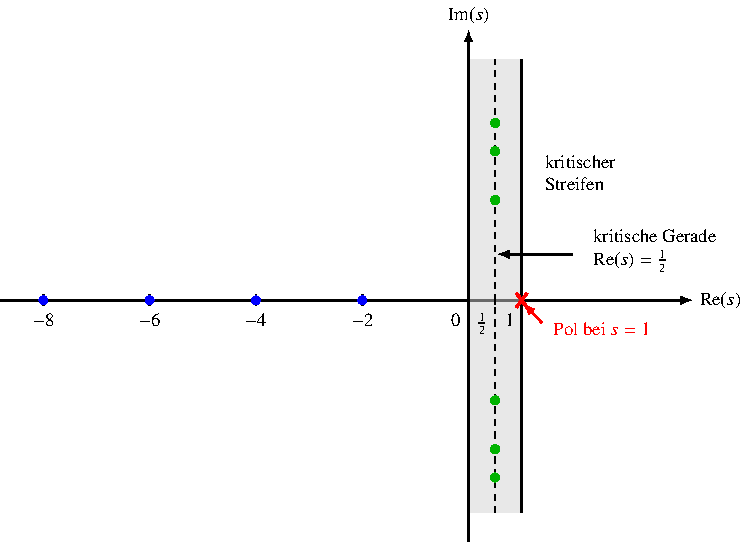
\includegraphics{papers/hankel/images/nullstellen.pdf}
%	
%	\begin{tikzpicture}[x=0.9cm,y=0.12cm,font=\small,>=latex]
%		
%		% ------------------------------------------------------------
%		% Achsen
%		% ------------------------------------------------------------
%		\draw[->] (-8.8,0) -- (4.2,0) node[right] {$\Re(s)$};
%		\draw[->] (0,-34) -- (0,38) node[above] {$\Im(s)$};
%		
%		% ------------------------------------------------------------
%		% Kritischer Streifen 0 < Re(s) < 1
%		% ------------------------------------------------------------
%		\fill[gray!18] (0,-30) rectangle (1,34);
%		\draw[thick] (0,-30) -- (0,34);
%		\draw[thick] (1,-30) -- (1,34);
%		
%		% kritische Gerade Re(s)=1/2
%		\draw[dashed,thick] (0.5,-30) -- (0.5,34);
%		
%		% ------------------------------------------------------------
%		% Markierungen auf der reellen Achse
%		% ------------------------------------------------------------
%		\foreach \x in {-8,-6,-4,-2,0,1}
%		{
%			\draw (\x,0.8) -- (\x,-0.8);
%		}
%		
%		\draw (0.5,0.6) -- (0.5,-0.6);
%		
%		\node[below] at (-8,-0.8) {$-8$};
%		\node[below] at (-6,-0.8) {$-6$};
%		\node[below] at (-4,-0.8) {$-4$};
%		\node[below] at (-2,-0.8) {$-2$};
%		
%		\node[below left]  at (0,-0.8) {$0$};
%		\node[below left]       at (0.5,-0.6) {$\frac12$};
%		\node[below left] at (1,-0.8) {$1$};
%		
%		% ------------------------------------------------------------
%		% triviale Nullstellen
%		% ------------------------------------------------------------
%		\foreach \x in {-8,-6,-4,-2}
%		{
%			\fill[blue] (\x,0) circle (2.1pt);
%		}
%		
%		%\node[align=center] at (-6.1,-12)
%		%{
%		%	triviale\\
%		%	Nullstellen
%		%};
%		
%		%\draw[->,green] (-5.95,-9.2) -- (-2.02,-0.5);
%		%\draw[->,green] (-5.95,-9.2) -- (-4.02,-0.5);
%		%\draw[->,green] (-5.95,-9.2) -- (-6.02,-0.5);
%		%\draw[->,green] (-5.95,-9.2) -- (-8.02,-0.5);
%		% ------------------------------------------------------------
%		% nichttriviale Nullstellen
%		% echte erste paar Ordinaten, alle auf Re(s)=1/2
%		% ------------------------------------------------------------
%		\foreach \y in {14.1347,21.0220,25.0109,-14.1347,-21.0220,-25.0109}
%		{
%			\fill[green!70!black] (0.5,\y) circle (2.2pt);
%		}
%		
%		% ------------------------------------------------------------
%		% Beschriftung kritischer Streifen
%		% ------------------------------------------------------------
%		\node[align=left] at (2.1,18)
%		{
%			kritischer\\
%			Streifen
%		};
%		
%		% kritische Gerade
%		\node[align=left] at (3.5,7)
%		{
%			kritische Gerade\\
%			$\Re(s)=\frac12$
%		};
%		
%		\draw[->] (1.95,6.5) -- (0.56,6.5);
%		
%		% nichttriviale Nullstellen
%		%\node[align=right] at (-1.5,23)
%		%{
%		%	nichttriviale\\
%		%	Nullstellen
%		%};
%		
%		%\draw[->,blue] (-0.55,21.5) -- (0.44,-14.1);
%		%\draw[->,blue] (-0.55,21.5) -- (0.44,-21.0);
%		%\draw[->,blue] (-0.55,21.5) -- (0.44,-25.0);
%		%\draw[->,blue] (-0.55,21.5) -- (0.44,25.0);
%		%\draw[->,blue] (-0.55,21.5) -- (0.44,21.0);
%		%\draw[->,blue] (-0.55,21.5) -- (0.44,14.1);
%		% ------------------------------------------------------------
%		% Pol bei s=1
%		% ------------------------------------------------------------
%		\draw[red,very thick] (0.90,-1.0) -- (1.10,1.0);
%		\draw[red,very thick] (0.90,1.0) -- (1.10,-1.0);
%		
%		\node[red,anchor=west] at (1.45,-4.0) {Pol bei $s=1$};
%		\draw[->,red] (1.38,-3.2) -- (1.05,-0.5);
%		
%	\end{tikzpicture}
	
	\caption{
		Darstellung der Nullstellen der Riemannschen Zetafunktion.
		Die \textcolor{blue}{trivialen Nullstellen} liegen bei den negativen geraden Zahlen.
		Der graue Bereich bezeichnet den kritischen Streifen \(0<\Re(s)<1\),
		die gestrichelte Linie die kritische Gerade \(\Re(s)=\tfrac12\).
		Die eingezeichneten ersten \textcolor{green!70!black}{nichttrivialen Nullstellen} liegen bei
		\(\tfrac12 \pm 14.1347\,i\),
		\(\tfrac12 \pm 21.0220\,i\) und
		\(\tfrac12 \pm 25.0109\,i\).
		Ausserdem besitzt \(\zeta(s)\) bei \(s=1\) einen einfachen Pol.
	}
	\label{hankel:fig:nullstellen}
\end{figure}

%\begin{figure}
%	\centering
%	
%	\begin{tikzpicture}[x=0.9cm,y=0.12cm,font=\small,>=latex]
%		
%		% ------------------------------------------------------------
%		% Achsen
%		% ------------------------------------------------------------
%		\draw[->] (-8.8,0) -- (4.2,0) node[right] {$\Re(s)$};
%		\draw[->] (0,-34) -- (0,38) node[above] {$\Im(s)$};
%		
%		% ------------------------------------------------------------
%		% Kritischer Streifen 0 < Re(s) < 1
%		% ------------------------------------------------------------
%		\fill[gray!18] (0,-30) rectangle (1,34);
%		\draw[thick] (0,-30) -- (0,34);
%		\draw[thick] (1,-30) -- (1,34);
%		
%		% kritische Gerade Re(s)=1/2
%		\draw[dashed,thick] (0.5,-30) -- (0.5,34);
%		
%		% ------------------------------------------------------------
%		% Markierungen auf der reellen Achse
%		% ------------------------------------------------------------
%		\foreach \x in {-8,-6,-4,-2,0,1}
%		{
%			\draw (\x,0.8) -- (\x,-0.8);
%		}
%		
%		\draw (0.5,0.6) -- (0.5,-0.6);
%		
%		\node[below] at (-8,-0.8) {$-8$};
%		\node[below] at (-6,-0.8) {$-6$};
%		\node[below] at (-4,-0.8) {$-4$};
%		\node[below] at (-2,-0.8) {$-2$};
%		
%		\node[below left]  at (0,-0.8) {$0$};
%		\node[below left]       at (0.5,-0.6) {$\frac12$};
%		\node[below left] at (1,-0.8) {$1$};
%		
%		% ------------------------------------------------------------
%		% triviale Nullstellen
%		% ------------------------------------------------------------
%		\foreach \x in {-8,-6,-4,-2}
%		{
%			\fill[blue] (\x,0) circle (2.1pt);
%		}
%		
%		%\node[align=center] at (-6.1,-12)
%		%{
%		%	triviale\\
%		%	Nullstellen
%		%};
%		
%		%\draw[->,green] (-5.95,-9.2) -- (-2.02,-0.5);
%		%\draw[->,green] (-5.95,-9.2) -- (-4.02,-0.5);
%		%\draw[->,green] (-5.95,-9.2) -- (-6.02,-0.5);
%		%\draw[->,green] (-5.95,-9.2) -- (-8.02,-0.5);
%		% ------------------------------------------------------------
%		% nichttriviale Nullstellen
%		% echte erste paar Ordinaten, alle auf Re(s)=1/2
%		% ------------------------------------------------------------
%		\foreach \y in {14.1347,21.0220,25.0109,-14.1347,-21.0220,-25.0109}
%		{
%			\fill[green!70!black] (0.5,\y) circle (2.2pt);
%		}
%		
%		% ------------------------------------------------------------
%		% Beschriftung kritischer Streifen
%		% ------------------------------------------------------------
%		\node[align=left] at (2.1,18)
%		{
%			kritischer\\
%			Streifen
%		};
%		
%		% kritische Gerade
%		\node[align=left] at (3.5,7)
%		{
%			kritische Gerade\\
%			$\Re(s)=\frac12$
%		};
%		
%		\draw[->] (1.95,6.5) -- (0.56,6.5);
%		
%		% nichttriviale Nullstellen
%		%\node[align=right] at (-1.5,23)
%		%{
%		%	nichttriviale\\
%		%	Nullstellen
%		%};
%		
%		%\draw[->,blue] (-0.55,21.5) -- (0.44,-14.1);
%		%\draw[->,blue] (-0.55,21.5) -- (0.44,-21.0);
%		%\draw[->,blue] (-0.55,21.5) -- (0.44,-25.0);
%		%\draw[->,blue] (-0.55,21.5) -- (0.44,25.0);
%		%\draw[->,blue] (-0.55,21.5) -- (0.44,21.0);
%		%\draw[->,blue] (-0.55,21.5) -- (0.44,14.1);
%		% ------------------------------------------------------------
%		% Pol bei s=1
%		% ------------------------------------------------------------
%		\draw[red,very thick] (0.90,-1.0) -- (1.10,1.0);
%		\draw[red,very thick] (0.90,1.0) -- (1.10,-1.0);
%		
%		\node[red,anchor=west] at (1.45,-4.0) {Pol bei $s=1$};
%		\draw[->,red] (1.38,-3.2) -- (1.05,-0.5);
%		
%	\end{tikzpicture}
%	
%	\caption{
%		Darstellung der Nullstellen der Riemannschen Zetafunktion.
%		Die \textcolor{blue}{trivialen Nullstellen} liegen bei den negativen geraden Zahlen.
%		Der graue Bereich bezeichnet den kritischen Streifen \(0<\Re(s)<1\),
%		die gestrichelte Linie die kritische Gerade \(\Re(s)=\tfrac12\).
%		Die eingezeichneten ersten \textcolor{green!70!black}{nichttrivialen Nullstellen} liegen bei
%		\(\tfrac12 \pm 14.1347\,i\),
%		\(\tfrac12 \pm 21.0220\,i\) und
%		\(\tfrac12 \pm 25.0109\,i\).
%		Ausserdem besitzt \(\zeta(s)\) bei \(s=1\) einen einfachen Pol.
%	}
%	\label{hankel:fig:nullstellen}
%\end{figure}
\subsection{Die riemannsche Vermutung}

Riemann vermutete, dass sämtliche nichttrivialen Nullstellen auf der kritischen Geraden liegen~\cite{hankel:riemann}. 
\index{riemannsche Vermutung}%
Unter Ausschluss der trivialen Nullstellen lautet die Aussage
\begin{equation}
\boxed{
\zeta(s)=0
\quad\Longrightarrow\quad
\operatorname{Re}(s)=\frac{1}{2}
}
\label{hankel:eq:riemannsche-vermutung}
\end{equation}
für jede nichttriviale Nullstelle. 
Die Vermutung ist bis heute unbewiesen.
Ihre Bedeutung liegt in der engen Verbindung zwischen den Nullstellen der Zetafunktion und der Verteilung der Primzahlen. 
\index{Primzahlverteilung}%
Die analytische Fortsetzung ist dafür eine notwendige Voraussetzung.
Erst durch sie wird die Zetafunktion in dem Gebiet definiert, in dem diese Nullstellen liegen.

Die Bedeutung der riemannschen Vermutung reicht weit über die Zetafunktion selbst hinaus. 
David Hilbert nahm die Frage nach den Nullstellen der Zetafunktion im Jahr 1900 in Hilberts Liste mathematischer Probleme auf.
Hundert Jahre später wurde die riemannsche Vermutung vom Clay Mathematics Institute als eines der sieben Millennium-Probleme ausgewählt. 
\index{Millennium-Problem}%
Für ihre Lösung ist ein Preis von einer Million US-Dollar
ausgesetzt. 
Dass dieselbe Fragestellung über mehr als ein Jahrhundert
hinweg auf zwei der bekanntesten Listen mathematischer Probleme erscheint, unterstreicht ihre grundlegende Bedeutung für die Zahlentheorie.


